\input cinput.tex    \documentclass[12pt,fleqn,a4paper]{article}

\usepackage[style=newter5,citestyle=newter5,backend=biber,uniquename=false,natbib,maxnames=8]{biblatex}

\renewcommand{\bibfont}{\fontsize{12}{20pt}\selectfont}
\defbibheading{cjkhead}{\par\bigskip\bigskip\noindent{\large Reference}\par}


\usepackage{makeidx}
\usepackage{bm}
\usepackage{framed} % Easier way to use Framebox
\usepackage{pdfpages} % Import PDF in latex document
\usepackage{fancybox}
\usepackage{ulem} % for text strikethrough
\usepackage{listings} % For adding code
\usepackage{slashbox}
\usepackage{array}
\usepackage{enumitem}
\usepackage{amsmath, amssymb, amsthm}  % For mathematical symbols
\usepackage{rotating, booktabs}  % For table-rotating
\usepackage{longtable,booktabs}
\usepackage{wallpaper}  % For watermark
\usepackage{colortbl,color}
\usepackage{xcolor}
\usepackage{graphicx,psfrag}
\usepackage{tabularx,array}
\usepackage{booktabs}
\usepackage{multirow}
\usepackage{multicol}
\usepackage[subfigure]{tocloft}
\usepackage[tight]{subfigure}
\usepackage{float,booktabs,threeparttable}
\usepackage{caption}
\usepackage{menukeys}
\usepackage{longtable}
\usepackage{makeidx}
\usepackage{pdfpages}
\usepackage[refpage]{nomencl}



\addbibresource{chp_2.bib}


\def\se{{\rm se}}
%\newcommand{\red}{\color{red}}
\linespread{1.5}  % The linespread is 1.5.

% Define new theorem. ==============================================================
\newtheorem{thm}{Theorem}
\newtheorem{alg}{Algorithm}[section]  % Define new algorithm.
\newtheorem{definition}{Definition}
\newtheorem{lma}{\textbf{Lemma}}
\theoremstyle{definition}
\theoremstyle{plain}
% ===================================================================================

\setcounter{secnumdepth}{5}

\renewcommand{\contentsname}{Table of Contents}
\renewcommand{\listfigurename}{List of Figures}
\renewcommand{\listtablename}{List of Tables}
\renewcommand{\figurename}{\footnotesize Figure}
\renewcommand{\tablename}{\footnotesize Table}
\newcommand{\loflabel}{Figure}
\newcommand{\lotlabel}{Table}
\setlength{\abovecaptionskip}{0pt}

%\renewcommand{\cftsecpresnum}{Chapter }

\renewcommand{\cftsecnumwidth}{7em}
\renewcommand{\thesection}{{Chapter}~~ \arabic{section}}
\renewcommand{\thesubsection}{\arabic{section}.\arabic{subsection}}
\renewcommand{\thesubsubsection}{\arabic{section}.\arabic{subsection}.\arabic{subsubsection}}
% \renewcommand{\appendixpagename}{\Large\ctxfbb Appendix} % \ctxfb
\renewcommand{\arraystretch}{1.2}

%%%%%%%%%%

%%%%%%%%%%

\renewcommand{\nomname}{Notations}
\renewcommand*{\pagedeclaration}[1]{\unskip\dotfill\hyperpage{#1}}
\newcommand\independent{\protect\mathpalette{\protect\independenT}{\perp}}
\def\independenT#1#2{\mathrel{\rlap{$#1#2$}\mkern2mu{#1#2}}}
\makenomenclature

\makeindex

%\ctxfdef{\section}{\ctxfbb}
%\ctxfdef{\subsection}{\ctxfbb} %\ctxfr

\def\tb#1#2{\mathop{#1\vphantom{\sum}}\limits_{\displaystyle #2}}


% ======================== Set length ========================
\setlength{\columnsep}{2.4cm}
\setlength\parindent{0pt}
\textheight=22cm
\textwidth=16.5cm
\hoffset=-1cm
%\marginparwidth=0.5cm
% ============================================================

% Listings R Style ============================================================
\lstset{
frame=tb,
language=R,
showstringspaces=false,
columns=flexible,
keywordstyle=\color{blue},
commentstyle=\color{dkgreen},
stringstyle=\color{mauve},
%breaklines=true,
}



\begin{document}

\section{Statistical Learning}
\subsection{\textbf{Model}}
Often, our model can be illustrated as below
\begin{gather}
Y = f(X) + \epsilon
\end{gather}

Most of the time we can't get the true model $Y$ because the parameters for the predicator in $f(X)$ are unknown.
In this case, we need a prediction model to predict the response $Y$.
\begin{gather}
\hat{Y} = \hat{f}(X)
\end{gather}

As we can't measure the error term $\epsilon$, using $\hat{Y}$ to predict $Y$ is simply impossible.
Therefore, we need to do some transformation. This is so-called Population Regression Function.
\begin{gather}
E(Y) = E(f(X) + \epsilon) = f(X) \\
\hat{Y} = \hat{f}(X) \stackrel{Predict}{\longrightarrow} E(Y)=f(x)
\end{gather}

Note that $\epsilon \stackrel{i.i.d.}{\sim} \mathcal{N}(0,\sigma^{2}) $. So, $E(\epsilon)=0$.

\textbf{Notation}
\begin{itemize}
\item $Y$: the quantitative response of $Y$
\item $f(X)$: our model itself, where $X = (X_{1},X_{2},X_{3},\dots,X_{p})$ with $p$ different predictors
\item $\epsilon$: Random error term, in linear regression $\epsilon \stackrel{i.i.d.}{\sim} \mathcal{N}(0,\sigma^{2}) $ as an assumption
\end{itemize}


\subsection{\textbf{Assessing Model Accuracy}}
\subsubsection{\textbf{Measuring the Quality of Fit}}
In regression, the most common method to measure the fit of the data is the mean squared error(MSE), given by
\begin{gather}
MSE = \frac{1}{n}\sum\limits_{i=1}^{n}(y_{i}-\hat{f}(x_{i}))^2
\end{gather}
\begin{itemize}
\item Concept: Measuring the fit of training data
\item Goal: We are really not interested in whether $\hat{f}(x_{i}) \approx  y_{i}$; instead we want to know whether $\hat{f}(x_{0}) \approx y_{0}$, where $(x_{0},y_{0})$ is an unseen test observation not used to train the model.
\end{itemize}


\subsubsection{\textbf{The Bias-Variance Trade-Off}}

\begin{figure}[H]
\centering
\psfrag{A}[cl][c]{\tiny linear regression model}
\psfrag{B}[cl][c]{\tiny smoothing spline($p=5$)}
\psfrag{C}[cl][c]{\tiny smoothing spline($p=20$)}
\psfrag{D}[cl][c]{\tiny testing MSE}
\psfrag{E}[cl][c]{\tiny training MSE}
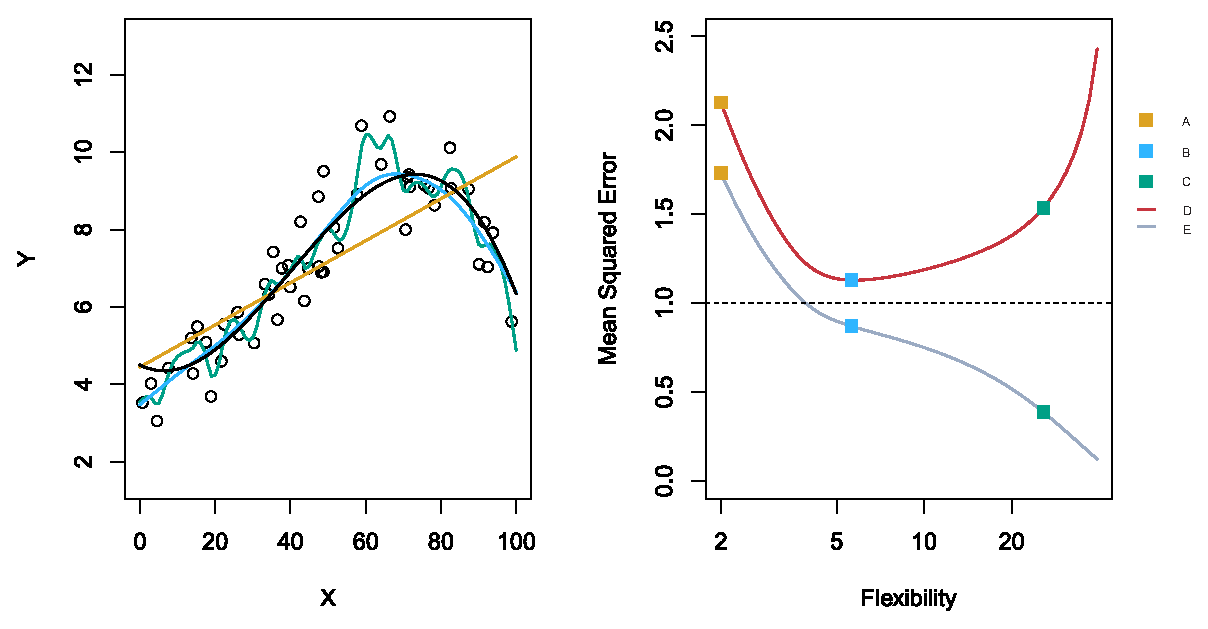
\includegraphics[scale=0.7]{images//2_9.eps}
\\~\\
\caption{The black curve represents the true model $f$. The other curves are $\hat{f}$ which are used to predict $E(f)$.}\label{figure-2.9}
\end{figure}

As shown in the figure above, when the flexibility grows the MSE of the testing data increases dramatically and turns into a U-curve.
The orange line is the linear regression fit, which is relatively inflexible. In the left hand panel of Figure~\ref{figure-2.9}, the blue and green curves are smoothing splines with different levels of flexibility.
As the model gets more flexible, it soon becomes over-fitted, making the MSE of test data increase. \\

The U-Shape observed in the test MSE curves turns out to be the result of two competing properties of statistical learning methods.
The MSE for a given $x_{0}$, can always be decomposed into the sum of three fundamental quantities:
the variance of $\hat{f}(x_{0})$, the square Bias of $\hat{f}(x_{0})$ and the variance for the error term $\epsilon$. That is,
\begin{align*}
E(y_{0}-\hat{f}(x_{0}))^{2} & = E(y_{0}^2)-2E(y_{0})E(\hat{f}(x_{0})) + E [\hat{f}(x_{0})^{2}] \\
& = E(f(x_{0})^2 + 2\epsilon f(x_{0})+\epsilon^{2})-2y_{0}E(\hat{f}(x_{0})) + E (\hat{f}(x_{0})^{2}) \\
& = f(x_{0})^2 + E(\epsilon^{2})-2y_{0}E(\hat{f}(x_{0})) + [\underline{E(\hat{f}(x_{0})^{2})- E [\hat{f}(x_{0})]^{2}}] + E [\hat{f}(x_{0})]^{2} \\
& = f(x_{0})^2-2y_{0}E(\hat{f}(x_{0}))+ E [\hat{f}(x_{0})]^{2} + Var(\hat{f}(x_{0}))+Var(\epsilon) \\
& = [E(\hat{f}(x_{0}))-f(x_{0})]^{2}+ Var(\hat{f}(x_{0}))+Var(\epsilon) \\
& = [Bias(\hat{f}(x_{0}))]^{2}+ Var(\hat{f}(x_{0}))+Var(\epsilon)
\end{align*}

\begin{framed}
\textbf{Unbiased Estimator and Bias}\\
----------------------------------------- \\
$\hat{\theta}\stackrel{estimate}{\longrightarrow} \theta $ \\
$E(\hat{\theta})= \theta$ \\
${\rm Bias}(\hat{\theta}) = E(\hat{\theta}) - \theta $ \\
----------------------------------------- \\
$\hat{f}(x)\stackrel{estimate}{\longrightarrow} f(x)$\\
$E(\hat{f}(x))= f(x)$ \\
${\rm Bias}(\hat{f}(x)) = E(\hat{f}(x)) - f(x) $ \\
\end{framed}


\begin{figure}[H]
\centering
\psfrag{A}[cl][c]{\tiny linear regression model}
\psfrag{B}[cl][c]{\tiny smoothing spline($p=3$)}
\psfrag{C}[cl][c]{\tiny smoothing spline($p=22$)}
\psfrag{D}[cl][c]{\tiny testing MSE}
\psfrag{E}[cl][c]{\tiny training MSE}
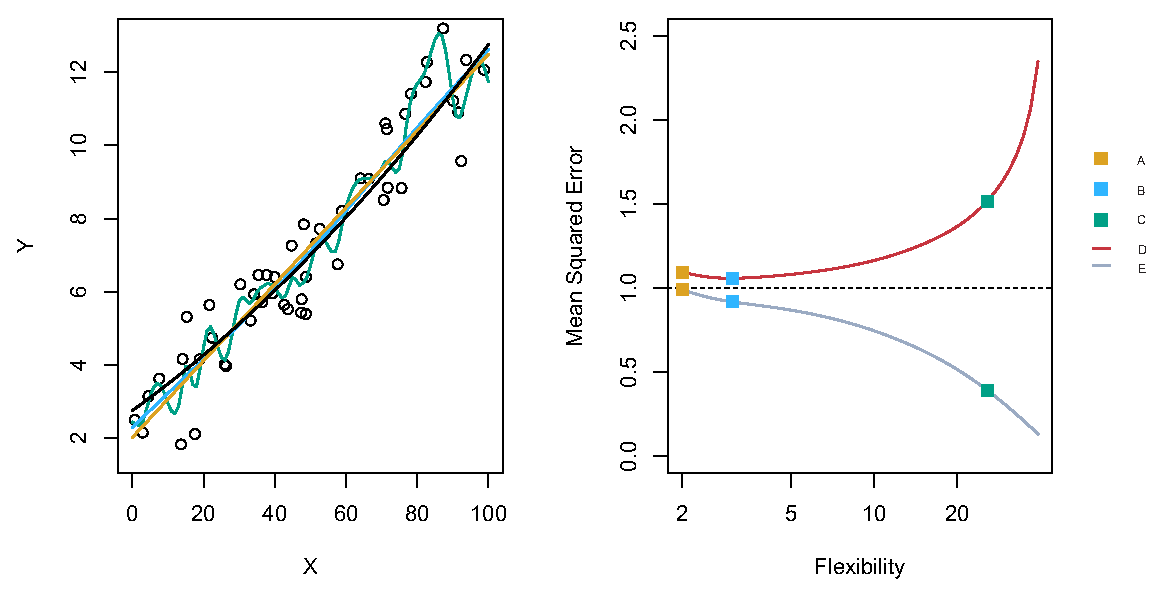
\includegraphics[scale=0.7]{images//2_10.eps}
\\~\\
\caption{Anthother $f$ which is closer to linear. The black curve in the left panel is the true $f(X)$. In this setting, linear regression provides a good fit to the data.}\label{figure-2.10}
\end{figure}


\begin{figure}[H]
\centering
\psfrag{A}[cl][c]{\tiny linear regression model}
\psfrag{B}[cl][c]{\tiny smoothing spline($p=10$)}
\psfrag{C}[cl][c]{\tiny smoothing spline($p=22$)}
\psfrag{D}[cl][c]{\tiny testing MSE}
\psfrag{E}[cl][c]{\tiny training MSE}
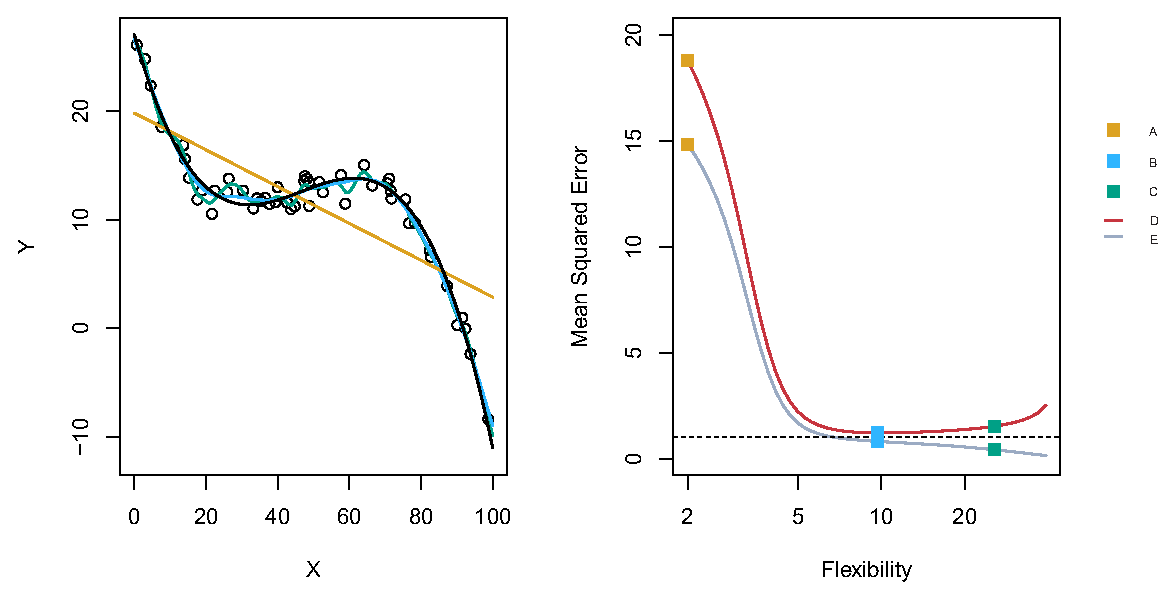
\includegraphics[scale=0.7]{images//2_11.eps}
\\~\\
\caption{Anthother $f$ which is far from linear. In this setting, linear regression provides a poor fit to the data.}\label{figure-2.11}
\end{figure}

\begin{itemize}
\item Variance : refers to the amount by which $\hat{f}$ would change if we estimated it using a different training data set.
\item Bias: refers to the error that is introduced by approximating $f$
\end{itemize}

As a general rule, the more flexible models gets, the variance increases and the more the bias decrease.

\begin{figure}[H]
\centering
\psfrag{A}[c][c]{\footnotesize Figure~\ref{figure-2.9}}
\psfrag{B}[c][c]{\footnotesize Figure~\ref{figure-2.10}}
\psfrag{C}[c][c]{\footnotesize Figure~\ref{figure-2.11}}
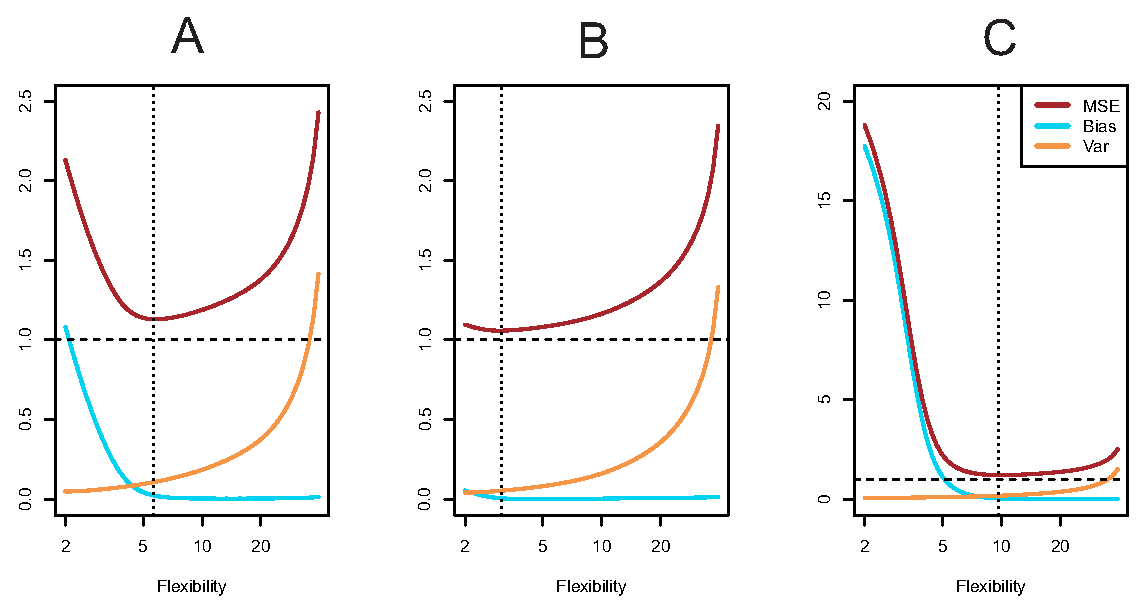
\includegraphics[scale=0.7]{images//2_12.eps}
\\~\\
\caption{Square Bias(Blue Curve), Variance(Orange Curve) and MSE(Red Curve) from test data of Figure~\ref{figure-2.9}, Figure~\ref{figure-2.10} and Figure~\ref{figure-2.11}.}\label{figure-2.12}
\end{figure}

The Figure~\ref{figure-2.12} represents the trade-off of variance and bias. Good statistical learning model requires low variance as well as low squared bias for the test data.
However, in general, the bias decreases and the variance increases as the flexibility(dimension) of the model increases. \\
~\\
Most of the time in a real-life situation $f$ is unknown, it is impossible to compute the test MES, bias, or the variance for a learning model.
Nevertheless, one should always keep the bias-variance trade-off in mind.


\subsubsection{\textbf{Classification Settings}}
Estimate $f$ on the basis of training observations ${(x_{1},y_{1}),\dots,(x_{n},y_{n})}$, where $y_{1},\dots,y_{n}$ are qualitative response.
$\hat{f}$ is the training error rate, the proportion of mistakes :
\begin{gather}
\hat{f} = \frac{1}{n}\sum\limits_{i=1}^{n}I(y_{i}\neq \hat{y}_{i})
\end{gather}

$\hat{y}_{i}$: the predicted class label for the $i$th observation
\begin{gather}
I(y_{i}\neq \hat{y}_{i}) = \left\{
\begin{array}{ll}
1, & y_{i}\neq \hat{y}_{i}\\
0, & y_{i}=\hat{y}_{i}\\
\end{array} \right.
\end{gather}


\subsubsection{\textbf{The Bayes Classifier}}

More detail in Chapter 4.4

\subsubsection{\textbf{Linear Models and Least Squares}}
\begin{gather}
\hat{Y} = X^{T}\hat{\beta} \\
{\rm RSS}(\beta) = \sum\limits_{i=1}^{N} (y_{i}-x_{i}^{T}\beta)^{2} \\
{\rm f.o.c}~~ \frac{\partial {\rm RSS}(\beta)}{\partial \beta} = \mathbf{X}^{T}(\mathbf{y}-\mathbf{X}\beta)=0 \\
\hat{\beta} = (\mathbf{X}^{T}\mathbf{X})^{-1}\mathbf{X}^{T}\mathbf{y}
\end{gather}

\begin{framed}
\textbf{R code:}
\begin{lstlisting}[language=R]
x = matrix(c(1,1,1,1,1,1,0.35,0.475,0.56,0.54,0.61,0.59),nrow = 6, ncol = 2)
y = matrix(c(4,5.25,6.8,6.45,7.8,7.55),nrow = 6, ncol = 1)
fit1 = lm(y ~ x)
solve((t(x) %*% x)) %*% (t(x) %*% y)
\end{lstlisting}
\end{framed}


\subsubsection{\textbf{Nearest-Neighbour Methods: to predict a quantitative response}}
The models is defines as follows:
\begin{gather}
\hat{Y}(x)=\frac{1}{k}\sum\limits_{x_{i}\in N_{k}(x)} y_{i}
\end{gather}

\begin{itemize}
\item Concept : average $k$ training points $x_{i}$ nearest to $x$
\item $N_{k}$: the neighbourhood of $x$ defined by the $k$ closest points $x_{i}$ in the training sample $\mathcal{T}$
\item $x_{i}$: represent the training data in input space, $i=1,2,3,...,N$
\end{itemize}

Implementation:
\begin{itemize}
\item Step 1: Choose data point $x$
\item Step 2: Find the $k$ observations with $x_{i}$ closest(Euclidean Distance) to $x$ in input space and average their response to get $\hat{Y}(x)$
\item Step 3: Move to the next data point and repeat above
\end{itemize}


\subsubsection{\textbf{Nearest-Neighbour Methods: to predict a qualitative response}}
The models is defines as follows:
\begin{gather}
{\rm Pr}(Y=j|X=x_{0}) = \frac{1}{K}\sum\limits_{i \in N_{0}}I(y_{i}=j)
\end{gather}

\begin{itemize}
\item $\sum\limits_{i \in N_{0}}I(y_{i}=j)$ : Summarize $k$ points nearest to $x_{0}$ according to class $j$
\end{itemize}

\begin{framed}
Example: \\
k-Nearest Neighbour ($k=3$)

\begin{figure}[H]
\centering
\psfrag{A}[c][c]{$x_{0}$}
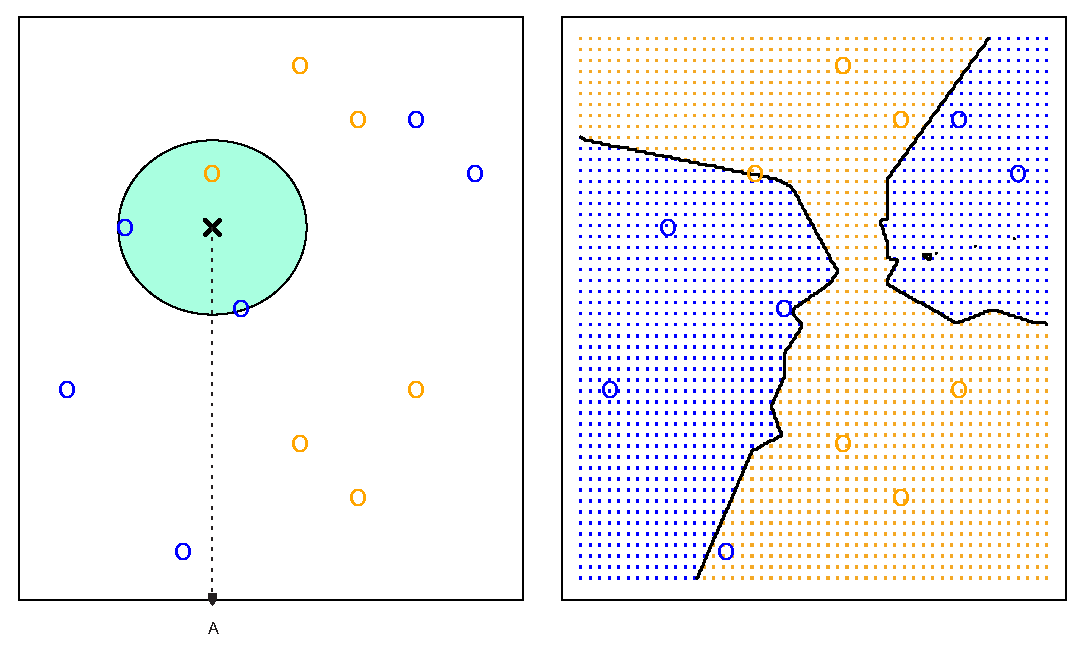
\includegraphics[scale=0.5]{images//2_14.eps}
\\~\\
\end{figure}

\begin{gather}
{\rm Pr}(Y=j|X=x_{0}) = \left\{
\begin{array}{ll}
\frac{1}{K}\sum\limits_{i \in N_{0}}I(y_{i}=\mbox{Blue}), & j = \mbox{\color{blue}Blue}\\
\frac{1}{K}\sum\limits_{i \in N_{0}}I(y_{i}=\mbox{Orange}), & j = \mbox{\color{orange}Orange}\\
0, & \mbox{otherwise}
\end{array} \right.
\end{gather}

\begin{gather}
{\rm Pr}(Y=j|X=x_{0}) = \left\{
\begin{array}{ll}
\frac{1}{3}\sum\limits_{i \in N_{0}}I(y_{i}=\mbox{Blue}) = \frac{2}{3}, & j = \mbox{\color{blue}Blue}\\
\frac{1}{3}\sum\limits_{i \in N_{0}}I(y_{i}=\mbox{Orange})= \frac{1}{3}, & j = \mbox{\color{orange}Orange}\\
0, & \mbox{otherwise} \\
\end{array} \right.
\end{gather}

Inference: \\
The probability for Blue circle ($2/3$) is higher than Orange circle ($1/3$). The test data $x_{0}$ should be classified as  Blue circle.

\end{framed}
%=====================================================================================================================================================
\subsection{\textbf{Exercises}}
%=====================================================================================================================================================
\begin{enumerate}
\item[1.] For each of parts (a) through (d), indicate whether we would generally
expect the performance of a flexible statistical learning method to be
\underline{better or worse} than an inflexible method. Justify your answer.
    \begin{enumerate}
        \item The sample size $n$ is extremely large, and the number of predictors $p$ is small.
        \item The number of predictors $p$ is extremely large, and the number of observations $n$ is small.
        \item The relationship between the predictors and response is highly non-linear.
        \item The variance of the error terms, i.e. $\sigma^{2} = {\rm Var}(\epsilon)$, is extremely high.
    \end{enumerate}
\end{enumerate}

\begin{framed}
Answer:
    \begin{enumerate}
        \item[(a)] Better. If we have sufficient data, then it's better to fit a flexible model, since we can picture our true model easily with large dataset.
        \item[(b)] Worse. If we fit a flexible model with the number of observations is small, it'll course over-fitting.
        \item[(c)] Better. A non-linear model consists of high dimension. This property makes the model more flexible.
        \item[(d)] Worse. When a model with a high $\sigma^{2}$, then it's better to apply a inflexible model to control the variance.
    \end{enumerate}
\end{framed}

%=====================================================================================================================================================

\begin{enumerate}
\item[2.] Explain whether each scenario is a \underline{\textbf{classification or regression}} problem,
and indicate whether we are most interested in \underline{\textbf{inference or prediction}}. Finally, provide \underline{\textbf{$n$ and $p$}}.
    \begin{enumerate}
        \item We collect a set of data on the top 500 firms in the US. For each firm we record profit, number of employees, industry and the CEO salary.
              We are interested in understanding which factors affect CEO salary.
        \item We are considering launching a new product and wish to know whether it will be a success or a failure.
              We collect data on 20 similar products that were previously launched.
              For each product we have recorded whether it was a success or failure, price charged for the product, marketing budget, competition price, and ten other variables.
        \item We are interesting in predicting the \% change in the US dollar in relation to the weekly changes in the world stock markets.
              Hence we collect weekly data for all of 2012. For each week we record the \% change in the dollar, the \% change in the US market, the \% change in the British market,
              and the \% change in the German market.
    \end{enumerate}
\end{enumerate}

\begin{framed}
Answer:
    \begin{enumerate}
        \item[(a)]
            \begin{itemize}
                \item Regression problem, since we want to know which predicator effect the CEO salary the most.
                \item Inference
                \item $n=500$
                \item $p$:profit, number of employees and industry
                \item Response: the CEO salary
            \end{itemize}
        \item[(b)]
            \begin{itemize}
                \item Classification problem, since we make use of the previous data to predict whether the new product will success of not.
                \item Prediction
                \item $n=20$
                \item $p$: price charged for the product, marketing budget, competition price, and ten other variables
                \item Response: success or failure
            \end{itemize}
        \item[(c)]
            \begin{itemize}
                \item Regression problem, since we want to predict \% change in the US dollar
                \item Prediction
                \item $n=52$
                \item $p$: the \% change in the US dollar, the \% change in the British market, and the \% change in the German market.
                \item Response: \% change in the US dollar
            \end{itemize}
    \end{enumerate}
\end{framed}

%=====================================================================================================================================================

\begin{enumerate}
\item[7.] The table below provides a training data set containing six observations, three predictors, and one qualitative response variable.

\begin{table}[H]
\centering
\begin{tabular}{lllll}
Obs.  & $X_{1}$    & $X_{2}$     & $X_{3}$  & $Y$ \\
\toprule
1 & 0 & 3 & 0 & Red \\
2 & 2 & 0 & 0 & Red \\
3 & 0 & 1 & 3 & Red \\
4 & 0 & 1 & 2 & Green \\
5 & -1 & 0 & 1 & Green \\
6 & 1 & 1 & 1 & Red \\
\bottomrule
\end{tabular}
\end{table}
Suppose we wish to use this data set to make a prediction for Y when $X_{1} = X_{2} = X_{3} = 0$ using K-nearest neighbours.
    \begin{enumerate}
        \item Compute the Euclidean distance between each observation and the test point, $X_{1} = X_{2} = X_{3} = 0$
        \item What is our prediction with K = 1? Why?
        \item What is our prediction with K = 3? Why?
        \item If the Bayes decision boundary in this problem is highly non-linear, then would we expect the best value for K to be large or small? Why?
    \end{enumerate}
\end{enumerate}

\begin{framed}
Answer:
    \begin{enumerate}
        \item[(a)]
            \begin{tabular}{llllll}
            Obs.  & $X_{1}$    & $X_{2}$     & $X_{3}$  & $Y$ & Euclidean\\
            \toprule
            $x_{0}$ & 0 & 0 & 0 & &  \\
            \toprule
            1 & 0 & 3 & 0 & Red & 3 \\
            2 & 2 & 0 & 0 & Red & 2 \\
            3 & 0 & 1 & 3 & Red & 3.16 \\
            4 & 0 & 1 & 2 & Green & 2.23 \\
            5 & -1 & 0 & 1 & Green & 1.41 \\
            6 & 1 & 1 & 1 & Red & 1.73 \\
            \bottomrule
            \end{tabular}
        \item[(b)] If K=1, then the category of obs.5 will be the most similar one, since the closest distance. The prediction of $\hat{f}(x_{0})$ will be Green

        \item[(c)] If K=3, we'll choose the top 3 data points which are closest to $x_{0}$. In this case, obs.5, obs.6 and obs.2 will be selected. The probability can be illustrated as below:
            \begin{gather}
            {\rm Pr}(Y=j|X=x_{0}) = \left\{
            \begin{array}{ll}
            \frac{1}{3}\sum\limits_{i \in (5,6,2)}I(y_{i}=\mbox{Red}) = \frac{2}{3}, & j = \mbox{\color{red}Red}\\
            \frac{1}{3}\sum\limits_{i \in (5,6,2)}I(y_{i}=\mbox{Green})= \frac{1}{3}, & j = \mbox{\color{green}Green}\\
            0, & \mbox{otherwise} \\
            \end{array} \right.
            \end{gather}
            Since, $x_{0}$ is more likely to be Red according to higher probability ($\frac{2}{3}$). We'll predict $x_{0}$ as Red.
        \item[(d)] If the problem is highly non-linear, K should be small. Due to KNN's property, when k is small it means the model is more flexible
                   whereas a large K would try to fit a more linear boundary because it takes more points into consideration.
    \end{enumerate}
\end{framed}

\section*{Reference}
\noindent
\begin{description}\itemsep=-2pt
\item {\MbQ\cH34}\z{\MiQ\cH16} (2012), {\MaQ\cH7}{\MbQ\cH84}\z{\MhQ\cH229}\z{\MeQ\cH78}\z{\McQ\cH228}\z{\MaQ\cH231}\z{\McQ\cH36}\z{\McQ\cH108}{\MaQ\cH8}, {\McQ\cH251}\z{\MhQ\cH23}, {\MkQ\cH49}\z{\MiQ\cH95}\z{\MaQ\cH199}\z{\MbQ\cH122}
\item Friedman, J., Hastie, T., \& Tibshirani, R. (2001). {\it{The elements of statistical learning}} (Vol. 1). Springer, Berlin: Springer series in statistics.
\item James, G., Witten, D., Hastie, T., \& Tibshirani, R. (2013). {\it{An introduction to statistical learning}} (Vol. 6). New York: springer.
\item Wasserman, L. (2013). {\it{All of statistics: a concise course in statistical inference}}. Springer Science \& Business Media.
\end{description}


\fontsize{12}{20pt}\selectfont
\printbibliography[keyword=cjk,heading=cjkhead]
\renewcommand{\bibfont}{\fontsize{12}{15pt}\selectfont}
\printbibliography[notkeyword=cjk,heading=none]

\end{document}
